\documentclass{article}
\usepackage[utf8]{inputenc}
\usepackage[french]{babel}
\usepackage[T1]{fontenc}
\usepackage[hidelinks]{hyperref}

\usepackage{amsmath}
\usepackage{amssymb}
\usepackage{graphicx}
\usepackage{listings}
\usepackage{color}

\begin{document}

\begin{titlepage}
    \begin{center}
        
        {\Large Université de Mons}\\[1ex]
        {\Large Faculté Des Sciences}\\[1ex]
        
        \newcommand{\HRule}{\rule{\linewidth}{0.3mm}}
        % Title
        \HRule \\[0.5cm]
        { \LARGE \bfseries Réseaux 1 \\[0.3cm]}
        { \LARGE \bfseries Rapport : Selective Repeat \& Congestion \\[0.1cm]} % Commenter si pas besoin
        { \LARGE \bfseries Groupe 9 \\ [0.05cm]}
        \HRule \\[1.5cm]
        
        % Author and supervisor
        \begin{minipage}[t]{0.45\textwidth}
            \begin{flushleft} \large
                \emph{Professeur:}\\
                Bruno \textsc{Quoitin}\\
                \emph{Assistants:}\\
                Jeremy \textsc{Dubrulle}\\
            \end{flushleft}
        \end{minipage}
        \begin{minipage}[t]{0.45\textwidth}
            \begin{flushright} \large
                \emph{Auteurs:} \\
                Cyril \textsc{Moreau} (210376)\\
                Arnaud \textsc{Moreau} (211260)\\
            \end{flushright}
        \end{minipage}\\[2ex]
        
        \vfill
        
        % Bottom of the page
        \begin{center}
            \begin{tabular}[t]{c c c}
                
\includegraphics[height=1.5cm]{UMONS-Logo.jpg} &
                
\includegraphics[height=1.5cm]{FS-Logo.jpg} &
                %\hspace{0.3cm} &
            \end{tabular}
        \end{center}~\\
        
        {\large Année académique 2021-2022}
        
    \end{center}
\end{titlepage}

\newpage

\section{Construction et exécution}
\subsection{Simulateur}
Pour compiler le programme, veuillez exécuter la commande suivante dans le dossier racine :
\begin{verbatim}
    javac -d build reso/examples/selectiveRepeat/Demo.java
\end{verbatim}
Ensuite, pour exécuter le logiciel, veuillez exécuter la commande depuis le dossier \textit{build} créé :
\begin{verbatim}
    java reso/examples/selectiveRepeat/Demo
\end{verbatim}
Une fois l'application lancée, il faudra entrer le nombre de paquet à envoyer, la probabilité de perte
de paquet ou de acknowledgement, mais aussi le \textit{bit rate} du lien et la longeur du lien (en km).
\begin{figure}[h]
    \centering 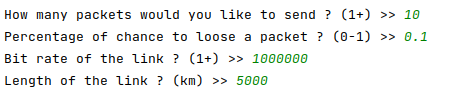
\includegraphics[scale=0.5]{data.png}
    \caption{Exemple de paramètres}
\end{figure}

\subsection{Création de plot pour la taille de la fenêtre}
Après avoir exécuté l'application, un fichier \emph{WindowSize.csv} est créé contenant
un historique des modifications de la taille de la fenêtre d'envoi.
Deux script python sont fournis afin de permettre de visualiser ces changement.
Le premier utilisant \emph{plotly} et le deuxième \emph{matplotlib}.
Afin de faire fonctionner ces script, veuillez installer les librairies suivantes : 
\begin{center}
    \begin{verbatim}
        pip install pandas
        pip install plotly (premier script)
        pip install matplotlib (deuxième script)
    \end{verbatim}
\end{center}
\textbf{Attention} le fichier \textit{WindowSize.csv} doit être dans le même dossier que le script.
Pour éxécuter un des script, il suffit d'exécuter l'une de ces commandes :
\begin{center}
    \begin{verbatim}
        python plot.py
        python plot2.py
    \end{verbatim} 
\end{center}

\newpage

\section{Approche utilisée dans l'implémentation}

\subsection{Selective repeat}
Après avoir implémenté la partie applicative en se basant sur l'exemple "ping-pong", 
nous avons commencé la partie Selective Repeat.
\vspace{0.5cm}

Tout d'abord, un choix a dû être effectué en ce qui concerne la fenêtre d'envoi. 
En effet, deux choix s'offraient à nous, soit utiliser une fenêtre exprimée en octet,
soit une fenêtre exprimée en packet.
C'est sur cette dernière possibilité que nous nous sommes basé. Il est beaucoup plus facile de gérer une fenêtre exprimée
en packet en java car il suffirait de délimiter la taille de la fenêtre entre deux indice d'un tableau de packet à envoyer.
Avec une fenêtre exprimée en octet, il faudrait vérifier la taille de chaque paquet ce qui rend la tâche plus compliquée.
Cette méthode a posé quelques problèmes lors de l'implémentation du contrôle de congestion décrite plus loin dans ce rapport.
\vspace{0.5cm}

Lorsque la taille de la fenêtre d'envoi diminue, il est possible que certains paquets ayant déjà été envoyés se retrouvent hors de la fenêtre d'envoi.
Afin de ne pas perdre ces paquets, les paquets déjà envoyés seront tout de même pris en compte même si ils ne sont plus dans la fenêtre d'envoi.


\subsection{Congestion control}
Comme précisé plus haut, le choix de modéliser la fenêtre d'envoi en paquet et non en octet a apporté quelques problèmes.
En effet, la formule permettant de calculer l'augmentation de la taille de la fenêtre lors du \textit{Additive Increase}
ne peut pas être utilisée directement.
\[
    cwnd' = cwnd + \frac{MSS^2}{cwnd}
\]
Dans la formule, le MSS est en octet mais notre fenêtre est exprimée en paquet nous avons donc dû adapter la formule à notre logiciel.
Sachant que le MSS vaut la taille maximale d'un paquet, nous avons donc remplacé cette valeur par 1.
Cependant, cela donnera une taille de fenêtre en nombre à virgule et non un entier. Nous avons donc converti la taille de la fenêtre
en double et calculons tout ce dont nous avons besoin sans arrondir cette valeur.
Cette valeur n'est uniquement arrondie que lorsque nous souhaitons envoyer un paquet et nous devons vérifier que ce paquet est dans la fenêtre d'envoi.
\[
    cwnd' = cwnd + \frac{1^2}{cwnd}
\]  

\newpage

\section{Difficultés rencontrées}
La difficulté majeure rencontrée a été que l'envoi de pacet successif ne s'effectuait pas, uniquement le dernier paquet était envoyé.
Nous avons donc essayé de contourner ce problème en créant une première méthode sendData permettant au sender d'envoyer ses données au protocol
qui les stockerait dans un buffer (créant au préalable un objet Packet) en essayant ensuite de les envoyer avec l'autre méthode sendData.

Nous avons Cependant trouvé la solution par la suite. Il suffisait simplement que les hôtes (host1 et host2) connaissent
les adresses MAC de l'autre ce qui evitait d'envoyer une requête ARP qui mettait le paquet en attente (Dans le simulateur, une seule requête ARP peut-être mise en attente. Si une nouvelle requête arrive, elle écrase la précédante)

\section{\'Etat de l'implémentation}
L'application est actuellement fonctionnelle dans la majeure partie des cas.
Cependant, lors de la réduction de la taille de la fenêtre, les packet qui étaient déjà envoyé et, à cause de cette réduction,
ne sont plus dans la fenêtre d'envoi continue à être utilisé. C'est finalement une bonne chose que les paquets ne soient pas perdus cependant, 
si un de ces paquets n'a pas été envoyé (donc appel à \emph{timeout()}) le paquet est directement renvoyé alors qu'il ne fait pas partie de la fenêtre.

\end{document}